%package list
\documentclass{article}
\usepackage[top=3cm, bottom=3cm, outer=3cm, inner=3cm]{geometry}
\usepackage{graphicx}
\usepackage{url}
%\usepackage{cite}
\usepackage{hyperref}
\usepackage{array}
\usepackage{multicol}
\newcolumntype{x}[1]{>{\centering\arraybackslash\hspace{0pt}}p{#1}}
\usepackage{natbib}
\usepackage{pdfpages}
\usepackage{float}
\usepackage{multirow}
\usepackage[normalem]{ulem}
\useunder{\uline}{\ul}{}

\usepackage[english,spanish]{babel}
\usepackage[utf8]{inputenc}
\AtBeginDocument{\selectlanguage{spanish}}
\renewcommand{\figurename}{Figura}
\renewcommand{\refname}{Referencias}
\renewcommand{\tablename}{Tabla} %esto no funciona cuando se usa babel
\AtBeginDocument{%
	\renewcommand\tablename{Tabla}
}

\usepackage{fancyhdr}
\pagestyle{fancy}
\fancyhf{}
\setlength{\headheight}{30pt}
\renewcommand{\headrulewidth}{1pt}
\renewcommand{\footrulewidth}{1pt}
\fancyhead[L]{\raisebox{-0.2\height}{
\includegraphics[width=3cm]{img/logo_innovate}}}
\fancyhead[C]{}
\fancyhead[R]{\fontsize{12}{12}\selectfont	Convenio N$^{\circ}$ 165-INNOVATEPERU-PIEC1-2019}
\fancyfoot[L]{SISO}
\fancyfoot[C]{IIDSVA}
\fancyfoot[R]{Página \thepage}




\begin{document}
	
	\begin{center}	
		\fontsize{15}{15} \textbf{Informe de integración SISO-VID}
	\end{center}
	%\centerline{\textbf{\underline{\Large Título: Informe de revisión del estado del arte}}}
	%\vspace*{0.5cm}
	
	\begin{table}[h]
		\setlength{\tabcolsep}{0.5em} % for the horizontal padding
		{\renewcommand{\arraystretch}{1.6}% for the vertical padding
			\begin{tabular}{|p{4cm}|p{10.8cm}|}
				\hline 
				\textbf{Elaboración:} & Equipo técnico  \\	\hline 
				\textbf{Entidad Ejecutora:} & X-TRA PLUS SOLUCIONES DE ENERGÍA S.A.C  \\	\hline 
				\textbf{Proyecto:} & Desarrollo de un Sistema Adaptativo para la Detección de Somnolencia en Conductores de Transporte Interprovincial idóneo para las características únicas de las Carreteras del Perú mediante Sensado Híbrido utilizando Técnicas de Deep Learning.  \\	\hline 
				\textbf{Periodo:} & Marzo 2021  \\	\hline 
				\textbf{Fecha:} & \today  \\	\hline 
			\end{tabular}
		}
	\end{table}	
	
	
	
	\section{Objetivo}
	
	Implementar el modulo SISO-VID. Este componente de software es el encargado de detectar somnolencia a partir de una secuencia de video utilizando aprendizaje profundo.
	
	\section{Introducción}
	
	Según \textit{World Health Organization} \cite{who}, 1.24 millones de accidentes de tráfico ocurren cada día. Además, \textit{The National Highway Traffic Safety Administration} (NHTSA), menciono que en USA han ocurrido 153,297 accidentes de transito entre el 2011 al 2015, y de estos el 2.4\%  fueron causados por conductres con somnolencia. Incluso, 1.25 millones de personas mueren cada año en accidentes de transito, 20 a 50 millones han sido heridos o estan discapacitados y todo esto ha llegado a costar 518 billones de dolares. Mas alarmante, se predice que los accidentes de transito serán la quinta causa mas frecuente de muertes para el 2030 \citep{asirt}. \\
	

	Los principales métodos de detección de somnolencia pueden dividirse en 3 grandes grupos según \cite{ramzan2019survey}. El primer grupo esta conformado por los métodos basados en procesamiento de imágenes y video, estos métodos captan la señal a partir de una cámara y utilizando algoritmos de visión computacional logran detectar la somnolencia. El segundo grupo esta conformado por los métodos que utilizan sensores en el auto, estos sensores miden la fuerza de agarre del timon, los cambios en el tiempo de los angulos de giro e incluso analizan las señales de frecuencia cardiaca. El ultimo grupo, es muy intrusivo y se basan en medidas fisiológicas como el \textit{electroencephalogram} (EEG), \textit{electrooculogram} (EOG), \textit{electromyogram} (EMG) y \textit{electrocardiogram} (ECG).\\
	
	SISO-VID es un método basado en comportamiento, este modulo toma como entrada una secuencia de video y dectada si alguna escena de la secuencia de video presenta somnolencia. En resumen, se ha utilizado detección de rostros con una red neuronal \textit{Single Shot Detector} (SSD), luego sobre el rostro detectado se utilizó la red neuronal \textit{Inception} para detectar somnolencia. El método propuesto logro un 90\% de accuracy sonbre la base de datos SISO-IMG, esta base de datos fue creada especificamente para este proyecto (para mas detalles, puede revisar el informe de base de datos). 
	
	
	
	\section{Metodología de SISO-VID} \label{desarrollo}
	
	SISO-VID es un componente de software basado en aprendizaje profundo para la detección de somnolencia tomando como entrada una secuencia de video. En la Figura \ref{fig:siso_vid}, presentamos la metodología utilizada de SISO-VID. El método propuesto toma una secuencia de video como entrada, luego extrae los fotogramas, por cada fotograma se detecta el rostro utilizando la red neuronal SSD, para finalmente utilizar la red Inception sobre el rostro detectado para determinar si exista somnolencia.\\
	
	\begin{figure}[H]
		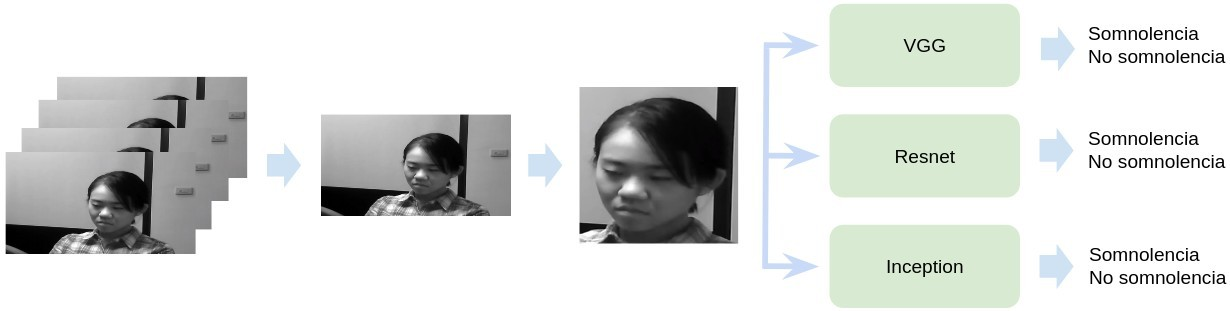
\includegraphics[width=\textwidth]{img/siso_vid}		
		\caption{Metodología utilizada por SISO-VID.}
		\label{fig:siso_vid}
	\end{figure}

	\subsection{Muestreo de fotogramas}
	
	El primer paso consiste en hacer un muestreo de la secuencia de video, es decir, tomando como entrada una secuencia de video, se extraen solo algunos fotogramas que serviran de entrada a los pasos siguientes (ver Figura \ref{fig:muestreo}). Se decide hacer este muestreo porque procesar todos los fotogramas demandaba mucho tiempo de procesamiento, considerando que SISO-VID opera en una Jetson Nano. Para el proyecto, se optó por hacer un muestreo de tres fotogramas cada segundo
	
		
	\begin{figure}[H]
		\centering
		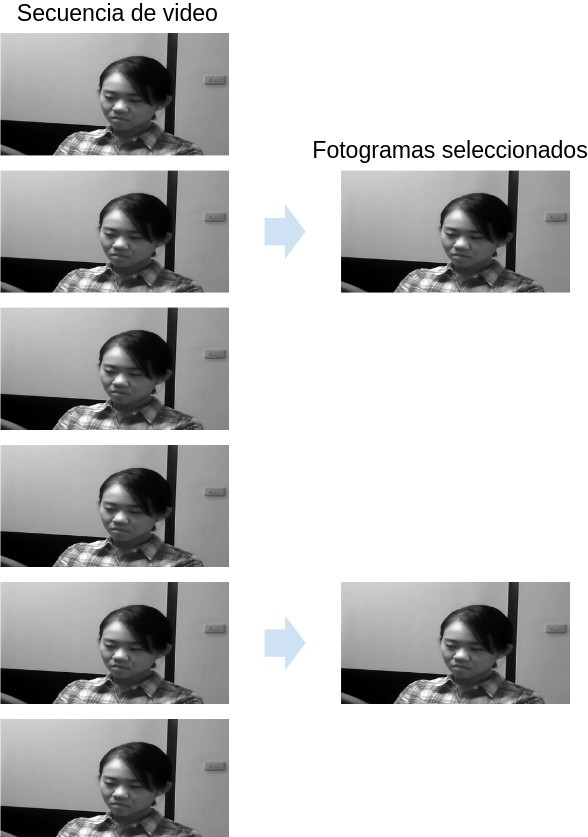
\includegraphics[width=0.4\textwidth]{img/muestreo}		
		\caption{Muestreo de los fotogramas en SISO-VID.}
		\label{fig:muestreo}
	\end{figure}
		
	
	\subsection{Detección de rostros}
	
	La detección de rostros consiste en obtener la posición  de un rostro dada como entrada una imagen. Por ejemplo, en la Figura \ref{fig:face}, tenemos una imagen, luego podemos aplicar algoritmos para obtener las coordenadas dentro de la imagen donde existan rostros, mayormente estas coordenadas son representadas con un rectangulo enfocando el rostro. 
	
	\begin{figure}[H]
		\centering
		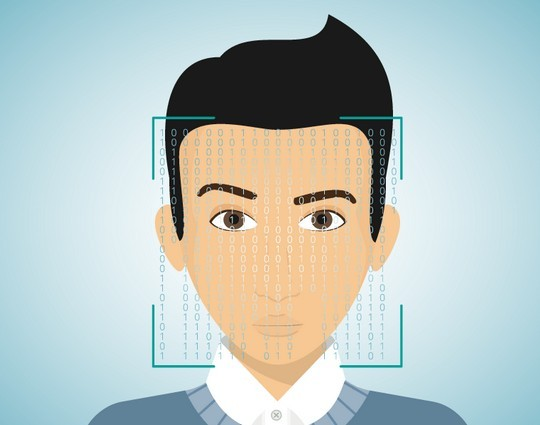
\includegraphics[width=0.4\textwidth]{img/face}		
		\caption{Ejemplo de detección de rostros.}
		\label{fig:face}
	\end{figure}

	Existen varios algoritmos de detección de rostros, uno de los primeros fue presentado por  \cite{viola2004robust}. Tambien existen algunas librerías, una de las mas utilizadas es \textit{dlib} \footnote{Librería de \textit{machine learning} y procesamiento de imágenes, desarrollada en C++. \href{http://dlib.net/}{Enlace}.}. Recientemente, se esta utilizando aprendizaje profundo para la detección de rostros, entre estas tenemos: \textit{Multi Task Convolutional Neural Netowrk} (MTCNN) \citep{zhang2016joint} y una red neuronal ya entrenada en OpenCV 3.0, basada en SSD e implementada en Caffe. Nosotros escogimos la segunda red neuronal, al ser la de mejor acierto.
	
	\subsection{Detección de somnolencia}
	
	Con cada rostro detectado en la etapa anterior, se evalua si este presenta o no somnolencia. En esta etapa se utilizo tres redes neuronales distintas: VGG, Inception y Resnet (ver Figura \ref{fig:drowsy}). Se escogieron estas redes al tener un buen desempeño en el estado del arte en clasificación de objetos. De las redes neuronales propuestas, el modelo Inception obtuvo los mejores resultados.
	
	\begin{figure}[H]
		\centering
		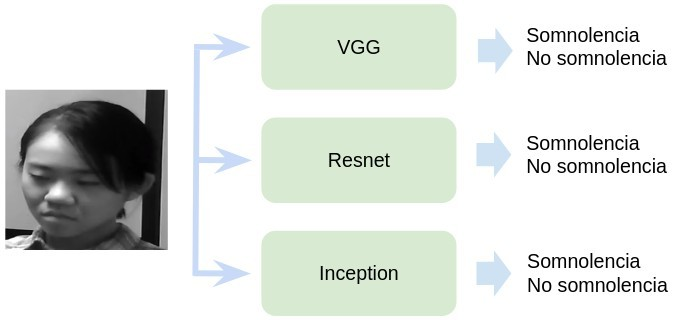
\includegraphics[width=0.6\textwidth]{img/drowsy}		
		\caption{Detección de somnolencia a partir de un rostro utilizando VGG, Resnet e Inception.}
		\label{fig:drowsy}
	\end{figure}
	
	La red neuronal Inception \cite{szegedy2016rethinking} en su tercera versión, es un modelo de reconocimiento de imágenes muy utilizado, está logro una exactitud de 78.1\% en la base de datos ImageNet. 
	
	\begin{figure}[H]
		\centering
		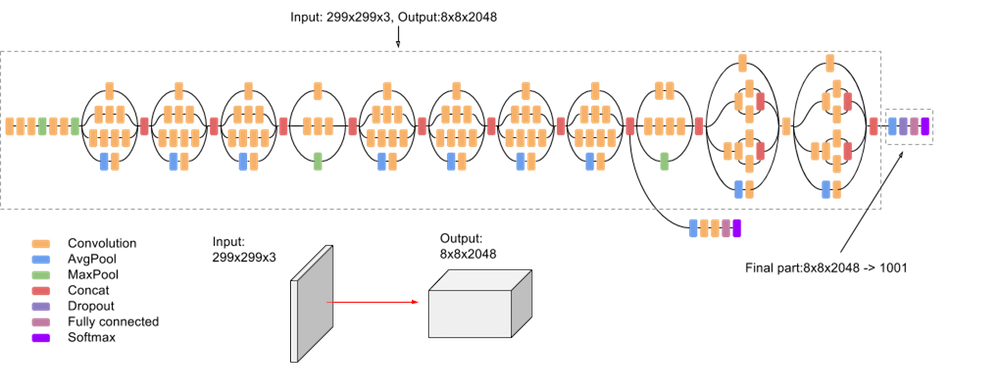
\includegraphics[width=\textwidth]{img/inception}		
		\caption{Detección de somnolencia a partir de un rostro utilizando VGG, Resnet e Inception.}
		\label{fig:drowsy}
	\end{figure}
	
	
	\section{Conclusiones y Recomendaciones}
	\begin{itemize}
		\item Se ha logrado revisar de los trabajos de mejor desempeño para la detección de somnolencia, estos han sido clasificados en 3 grupos, los basados en comportamiento, los basados en sensores del vehiculo y los fisiológicos. De estos, los de mejor desempeño son los fisiológicos, pero son intrusivos y los conductores no los utilizan. Los métodos basados en compartamiento son muy subseptibles a la ilumincación y cualquier atuendo que utilice el conductor que bloquee su rostro. En cambio los métodos basados en sensores en los vehiculos, parecen ser los menos intrusivos y con mayor posibilidad de exito.
		\item Tambien se ha confirmado la ausencia de una base de datos en la literatura en condiciones reales. Por ejemplo para el caso de los métodos basados en comportamiento, las bases de datos son secuencias de video grabadas en oficinas y en muchos casos, las acciones de somnolencia son actuadas; esto complica mucho la investigación en esta area, porque una escena real de un conductor presenta vibraciones del video y problemas de iluminación las cuales no estan presentes en las bases de datos utilizadas en la actualidad. Lo mismo sucede en los métodos que utilizan sensores en el vehiculo, la mayoria de trabajos han simulado la cabina del conductor y todas las  bases de datos son privadas.
		\item A pesar de que la detección de somnolencia sea un tema de investigación muy estudiado, es lamentable que en la literatura no se cuente con una base de datos en condiciones reales, donde los investigadores puedan evaluar sus algoritmos. Es verdad, que existen proyectos y empresas que cuentan con sistemas con un alto desempeño, pero las bases de datos son privadas y es imposible replicar sus resultados.		
	\end{itemize}



	%\clearpage
	
	\begin{table}[H]
	\begin{center}
			
	%\caption{Artículos de detección de somnolencia con procesamiento de video.}
	%\label{tab:comportameinto}
	\setlength{\tabcolsep}{0.5em} % for the horizontal padding
	{\renewcommand{\arraystretch}{1.4}% for the vertical padding
		
	\begin{tabular}{|p{1.6cm}|p{3cm}|p{3.5cm}|x{3.5cm}|p{2cm}|}
		\hline
		& \textbf{Nombre}    & \textbf{Cargo}         & \textbf{Firma} & \textbf{Fecha} \\ \hline
		\multirow{3}{1.6cm}{Elaborado por:} & Jason Paul Cahuana Nina        & Equipo técnico - Tesista La Salle    &  \raisebox{-.7\height}{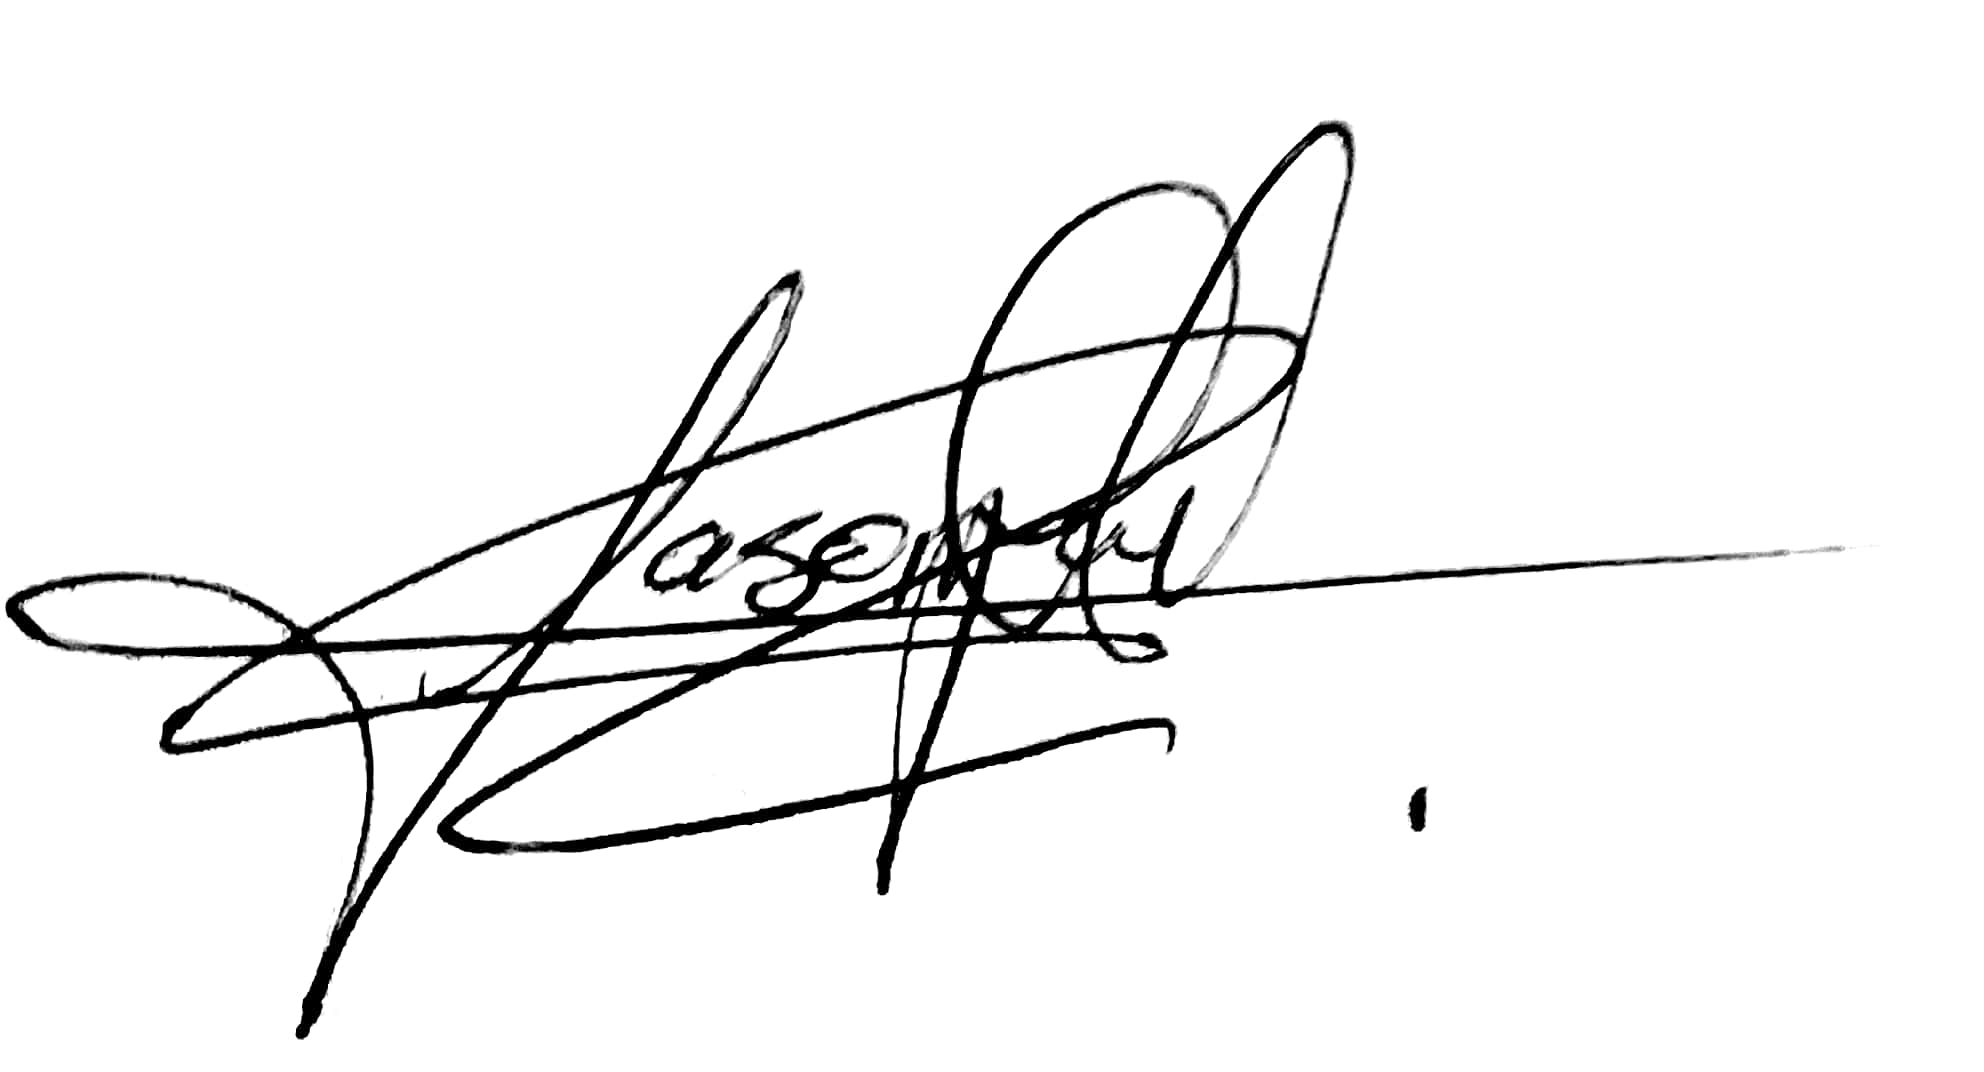
\includegraphics[width=2cm]{img/paul_firma.jpeg}}   &  12/03/2021     \\ \cline{2-5}		
		& Karla Mariel Fernández Fabián  & Investigador y desarrollador - Área de innovación y desarrollo tecnológico &  \raisebox{-.7\height}{
\includegraphics[width=2cm]{img/firma_KMFF}}     &   12/03/2021    \\ \hline
		
		& Vicente Enrique Machaca Arceda & Investigador y desarrollador - Área de innovación y desarrollo tecnológico &  \raisebox{-.7\height}{
\includegraphics[width=2cm]{img/firma_vicente}}     &   12/03/2021    \\ \hline
		
		\multirow{2}{1.6cm}{Revisado por:}  & Medardo Delgado Paredes        & Investigador La Salle  &  
			\raisebox{-.5\height}{
\includegraphics[width=2.5cm]{img/firma_yayo}}    &   12/03/2021    \\ \cline{2-5}	
		& Antonio Simon Bolivar Paredes  & Coordinador administrativo del proyecto    &     &  12/03/2021   \\ \hline
		Aprobado por:   & Elvis Diego Supo Colquehuanca  & Coorinador general del proyecto   &     &   12/03/2021   \\ \hline
	\end{tabular}

	}
	\end{center}
	\end{table}
	
	
	
	\clearpage
	\bibliographystyle{apalike}
	%\bibliographystyle{IEEEtranN}
	\bibliography{bibliography}
	
	
	\vspace*{\fill}
	
	

	
\end{document}
